% vim:set spell:
% vim:spell spelllang=fr:
\documentclass[a4paper]{article}
\usepackage[french]{babel}
\usepackage[utf8x]{inputenc}
\usepackage[T1]{fontenc}
\usepackage{libertine}
\usepackage[scaled=0.83]{beramono}
\usepackage{helvet}
\usepackage{graphicx}
\usepackage{amsmath,amssymb}
\usepackage[french]{babel}
\usepackage{xspace}
\usepackage{setspace}
\setstretch{1.0}
\usepackage{subfigure}
\voffset       -1in
\hoffset       -1in
\headheight     12pt
\headsep        12pt
\topmargin      25mm
\oddsidemargin  20mm
\textwidth      170mm
\textheight     240mm
\flushbottom
\graphicspath{{./figures/}{../../scripts/}}
\begin{document}
\begin{center}
\large
Travaux Pratiques Archi SLE-3A\\
Cours de Frédéric Pétrot\\
\LARGE
Implantations et évaluations de\\
quelques prédicteurs de branchements\\
\large

Durée~: 3 heures
\end{center}
\section{Organisation}
Ce TP se fait soit seul, soit en binôme, à votre convenance.
Le travail demandé TP fait l'objet d'un rendu contenant un court rapport qui inclut les \emph{résultats} d'expérimentations et un \emph{tarball} (ou un git) contenant vos sources à fournir en fin de séance.
Un gabarit en \LaTeX\ qui reprend le predicteur BHT avec un compteur à saturation est donné en exemple.
Vous avez également un script fourni pour vous permettre de systématiser les simulations et l'obtention des graphes des résultats.
Ce script marche avec le prédicteur BHT qui a deux arguments, il est donc nécessaire de le modifier pour l'utiliser avec un nombre d'arguments différent.

\section{Introduction}
On cherche à étudier le comportement en situation réelle de différents prédicteurs de branchement.
Pour cela, on va développer un modèle en C++ de chacun de ces prédicteurs sur lequel on fera passer un ensemble de traces d'exécutions et qui fournira en sortie le ratio de mauvaises prédictions (en fait le nombre de \emph{Miss Prediction per Kilo Instructions}, MPKI).
On fera varier les différents paramètres du prédicteur, en particulier la taille des tables, afin d'en extraire un comportement asymptotique (par benchmark), dont on tirera un graphe.

L'infrastructure dans laquelle insérer le modèle de prédicteur est celle qui a été utilisée par le \emph{The 5th JILP Championship Branch Prediction Competition (CBP-5)}\footnote{Dont on trouvera la version originale sur \texttt{https://www.jilp.org/cbp2016/framework.html}}.
Cette infrastructure effectue la lecture des traces et l'appel à des fonctions qui implantent le prédicteur, et donne en sortie diverses statistiques dont la valeur du MPKI.

Le prédicteur par défaut dans l'archive que je vous fournis est un prédicteur à saturation «~$n$-bits~» vu en cours et rappelé figure~\ref{2-bit} en considérant un prédicteur bimodal.
Dans une case donnée, un branchement «~prédit pris~» aura une valeur $v\geq 2^{n-1}$ et «~prédit non pris~» aura une valeur $v<2^{n-1}$.
Nous ferons en séance une analyse rapide du code afin de comprendre comment il a été implanté dans l'infrastructure.

\begin{figure}[htb]
   \begin{minipage}[t]{.44\linewidth}\vspace{0pt}
      \center\includegraphics[scale=1]{2-bits}
      \caption{Prédicteur bimodal}
      \label{2-bit}
   \end{minipage}%
\hfill
   \begin{minipage}[t]{.54\linewidth}\vspace{0pt}
      \center\includegraphics[scale=.65]{2bg1}
      \caption{\label{2bg1}Graphe de transitions du prédicteur bimodal}
   \end{minipage}
\end{figure}

\section{Travail demandé}
On implantera différents prédicteurs en prenant soin de paramétrer les tailles afin de pouvoir lancer facilement plusieurs exécutions (\emph{cf.} l'exemple fourni) et ainsi pouvoir tracer des courbes et voir les asymptotes.

Les prédicteurs que l'on pourra d'implanter sont les suivants~:
\begin{enumerate}
\item un prédicteur bimodal (ou $n$-modal) avec le graphe de transitions présenté figure~\ref{2bg1}.
      Notez la transition de NT à ST et de T à SNT, qui ne correspond pas à des transitions classiques du compteur à saturation;

\item un prédicteur global simple avec un historique des branchement de longueur (nombre de bits) $H$ permettant d'atteindre une entrée bimodale utilisant le graphe d'état n°1 (la \emph{Pattern History Table}).
      Pour mémoire, l'historique des branchements est un registre à décalage à gauche dans lequel on injecte sur le poids faible la décision prise ($H=3$ dans la figure~\ref{global-simple});
      \begin{figure}[hbt]\center\leavevmode
      \includegraphics[scale=.9]{global-simple}
      \caption{Prédicteur global simple}
      \label{global-simple}
      \end{figure}

\item un prédicteur \emph{gshare} qui est un prédicteur global pour lequel l'index définissant l'entrée dans la table de taille $2^n$ est calculé comme le ou-exclusif d'un registre d'historique avec le pc du branchement, comme illustré sur la figure~\ref{gshare};
      \begin{figure}[hbt]\center\leavevmode
      \includegraphics[scale=.9]{gshare}
      \caption{Prédicteur \emph{gshare}}
      \label{gshare}
      \end{figure}
      Si $H>n$, alors on prendra les $n$ bits de poids fort de $H$ pour faire le ou-exclusif;

\item un prédicteur corrélé qui utilise un historique sur $H$ bits permettant de sélectionner une PHT parmi $2^H$ et utilisant l'adresse du branchement pour indicer cette table, comme illustré sur la figure~\ref{correlated};
      \begin{figure}[hbt]\center\leavevmode
      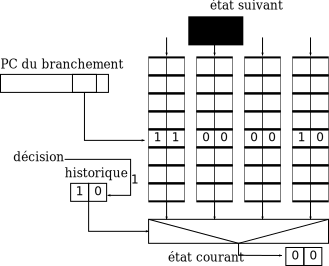
\includegraphics[scale=.9]{correlated}
      \caption{\label{correlated}Prédicteur corrélé}
      \end{figure}

\item un prédicteur local qui utilise une table d'historiques sur $H$ bits indexée par les poids faibles de l'adresse du branchement.  En utilisant l'entrée d'historique, on indice une PHT bimodale de taille $2^H$, comme illustré sur la figure~\ref{local};
      \begin{figure}[hbt]\center\leavevmode
      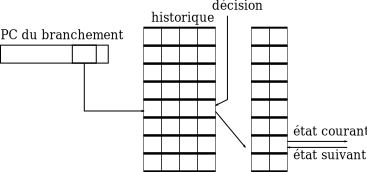
\includegraphics[scale=.9]{local}
      \caption{Prédicteur local}
      \label{local}
      \end{figure}

\item et pour finir un prédicteur mixte (celui de l'alpha 21264) qui utilise un prédicteur global simple avec un historique de $H_g=12$ (soit 4096 entrées), et un prédicteur local comme celui de la précédente question, avec $H_l=10$ par entrée de la table d'historique (soit 1024 entrées).
      La PHT indexée est un simple prédicteur de type bimodale, mais sur 3 bits, implantée avec un compteur à saturation.

      Le choix du prédicteur à utiliser se fait grâce à une BHT de 4K entrées de 2 bits.
      Le compteur est incrémenté lorsque le prédicteur \emph{prédit} est correcte et l'autre prédicteur a fait le mauvais choix, et est décrémenté dans le cas opposé (\emph{cf.} la machine d'état de la figure~\ref{mixte-graphe}).
      \begin{figure}[hbt]\center\leavevmode
      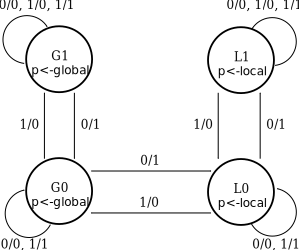
\includegraphics[scale=0.7]{mixte-graphe}
      \caption{Machine à états du choix du prédicteur.
      Légende~: $global/local$, $0$ décision incorrecte, $1$ décision correcte}
      \label{mixte-graphe}
      \end{figure}

      On ne tentera pas (du moins dans le temps imparti) de faire une version paramétrable de ce dernier prédicteur.
\end{enumerate}

Il y a un script \verb+sle3a-doit.sh+ dans le répertoire \verb+script+ qui lance automatiquement l'exécution sur un sous-ensemble des traces pour un prédicteur donné, qu'il a fallut préalablement compiler dans le répertoire \verb+sim+.
Il y a dans le script pour le prédicteur $n$-modal 2 boucles imbriquées~: la boucle externe, indice $i$, fait varier le nombre de bits du compteur, et la boucle interne, d'indice $j$, fait varier le nombre de bits de PC à utiliser pour indexer les tables.
Vous serez amené à modifier les valeurs des bornes en fonction des prédicteurs, voir à changer un peu cette partie si vous faite des prédicteurs exotiques.

Le script \verb+sle3a-doit.sh+ produit ses résultats dans \verb+../results/xxx+, ou \verb+xxx+ est un répertoire dont le nom peut-être choisi à l'envie.
Il les analyse ensuite et génère des programmes \texttt{python} qui servent à tracer des courbes (avec \texttt{matplotlib}).
Ce sont ces courbes que l'on vous demande d'analyser.

On donne sur la figure~\ref{results} le type de résultat attendu pour le prédicteur 1 bit.

      \begin{figure}[htb]
      \centering
      \subfigure[Table d'historique 1 bit]{
      \includegraphics[scale=.48]{graph_1}
      \label{plot1}
      }
      \subfigure[Table d'historique 2 bits]{
      \includegraphics[scale=.48]{graph_2}
      \label{plot2}
      }
      \subfigure[Table d'historique 3 bits]{
      \includegraphics[scale=.48]{graph_3}
      \label{plot3}
      }
      \subfigure[Table d'historique 4 bits]{
      \includegraphics[scale=.48]{graph_4}
      \label{plot4}
      }
      \subfigure[Table d'historique 5 bits]{
      \includegraphics[scale=.48]{graph_5}
      \label{plot3}
      }
      \subfigure[Table d'historique 6 bits]{
      \includegraphics[scale=.48]{graph_6}
      \label{plot4}
      }
      \caption{\label{results}Les courbes de MPKI}
      \end{figure}

Le sous-répetoire \verb+sle3a/rendu+ contient un exemple de .tex permettant de faire un petit rapport sur le travail.
\end{document}
